% Options for packages loaded elsewhere
\PassOptionsToPackage{unicode}{hyperref}
\PassOptionsToPackage{hyphens}{url}
%
\documentclass[
]{article}
\usepackage{amsmath,amssymb}
\usepackage{lmodern}
\usepackage{ifxetex,ifluatex}
\ifnum 0\ifxetex 1\fi\ifluatex 1\fi=0 % if pdftex
  \usepackage[T1]{fontenc}
  \usepackage[utf8]{inputenc}
  \usepackage{textcomp} % provide euro and other symbols
\else % if luatex or xetex
  \usepackage{unicode-math}
  \defaultfontfeatures{Scale=MatchLowercase}
  \defaultfontfeatures[\rmfamily]{Ligatures=TeX,Scale=1}
\fi
% Use upquote if available, for straight quotes in verbatim environments
\IfFileExists{upquote.sty}{\usepackage{upquote}}{}
\IfFileExists{microtype.sty}{% use microtype if available
  \usepackage[]{microtype}
  \UseMicrotypeSet[protrusion]{basicmath} % disable protrusion for tt fonts
}{}
\makeatletter
\@ifundefined{KOMAClassName}{% if non-KOMA class
  \IfFileExists{parskip.sty}{%
    \usepackage{parskip}
  }{% else
    \setlength{\parindent}{0pt}
    \setlength{\parskip}{6pt plus 2pt minus 1pt}}
}{% if KOMA class
  \KOMAoptions{parskip=half}}
\makeatother
\usepackage{xcolor}
\IfFileExists{xurl.sty}{\usepackage{xurl}}{} % add URL line breaks if available
\IfFileExists{bookmark.sty}{\usepackage{bookmark}}{\usepackage{hyperref}}
\hypersetup{
  hidelinks,
  pdfcreator={LaTeX via pandoc}}
\urlstyle{same} % disable monospaced font for URLs
\usepackage[margin=1in]{geometry}
\usepackage{color}
\usepackage{fancyvrb}
\newcommand{\VerbBar}{|}
\newcommand{\VERB}{\Verb[commandchars=\\\{\}]}
\DefineVerbatimEnvironment{Highlighting}{Verbatim}{commandchars=\\\{\}}
% Add ',fontsize=\small' for more characters per line
\usepackage{framed}
\definecolor{shadecolor}{RGB}{248,248,248}
\newenvironment{Shaded}{\begin{snugshade}}{\end{snugshade}}
\newcommand{\AlertTok}[1]{\textcolor[rgb]{0.94,0.16,0.16}{#1}}
\newcommand{\AnnotationTok}[1]{\textcolor[rgb]{0.56,0.35,0.01}{\textbf{\textit{#1}}}}
\newcommand{\AttributeTok}[1]{\textcolor[rgb]{0.77,0.63,0.00}{#1}}
\newcommand{\BaseNTok}[1]{\textcolor[rgb]{0.00,0.00,0.81}{#1}}
\newcommand{\BuiltInTok}[1]{#1}
\newcommand{\CharTok}[1]{\textcolor[rgb]{0.31,0.60,0.02}{#1}}
\newcommand{\CommentTok}[1]{\textcolor[rgb]{0.56,0.35,0.01}{\textit{#1}}}
\newcommand{\CommentVarTok}[1]{\textcolor[rgb]{0.56,0.35,0.01}{\textbf{\textit{#1}}}}
\newcommand{\ConstantTok}[1]{\textcolor[rgb]{0.00,0.00,0.00}{#1}}
\newcommand{\ControlFlowTok}[1]{\textcolor[rgb]{0.13,0.29,0.53}{\textbf{#1}}}
\newcommand{\DataTypeTok}[1]{\textcolor[rgb]{0.13,0.29,0.53}{#1}}
\newcommand{\DecValTok}[1]{\textcolor[rgb]{0.00,0.00,0.81}{#1}}
\newcommand{\DocumentationTok}[1]{\textcolor[rgb]{0.56,0.35,0.01}{\textbf{\textit{#1}}}}
\newcommand{\ErrorTok}[1]{\textcolor[rgb]{0.64,0.00,0.00}{\textbf{#1}}}
\newcommand{\ExtensionTok}[1]{#1}
\newcommand{\FloatTok}[1]{\textcolor[rgb]{0.00,0.00,0.81}{#1}}
\newcommand{\FunctionTok}[1]{\textcolor[rgb]{0.00,0.00,0.00}{#1}}
\newcommand{\ImportTok}[1]{#1}
\newcommand{\InformationTok}[1]{\textcolor[rgb]{0.56,0.35,0.01}{\textbf{\textit{#1}}}}
\newcommand{\KeywordTok}[1]{\textcolor[rgb]{0.13,0.29,0.53}{\textbf{#1}}}
\newcommand{\NormalTok}[1]{#1}
\newcommand{\OperatorTok}[1]{\textcolor[rgb]{0.81,0.36,0.00}{\textbf{#1}}}
\newcommand{\OtherTok}[1]{\textcolor[rgb]{0.56,0.35,0.01}{#1}}
\newcommand{\PreprocessorTok}[1]{\textcolor[rgb]{0.56,0.35,0.01}{\textit{#1}}}
\newcommand{\RegionMarkerTok}[1]{#1}
\newcommand{\SpecialCharTok}[1]{\textcolor[rgb]{0.00,0.00,0.00}{#1}}
\newcommand{\SpecialStringTok}[1]{\textcolor[rgb]{0.31,0.60,0.02}{#1}}
\newcommand{\StringTok}[1]{\textcolor[rgb]{0.31,0.60,0.02}{#1}}
\newcommand{\VariableTok}[1]{\textcolor[rgb]{0.00,0.00,0.00}{#1}}
\newcommand{\VerbatimStringTok}[1]{\textcolor[rgb]{0.31,0.60,0.02}{#1}}
\newcommand{\WarningTok}[1]{\textcolor[rgb]{0.56,0.35,0.01}{\textbf{\textit{#1}}}}
\usepackage{graphicx}
\makeatletter
\def\maxwidth{\ifdim\Gin@nat@width>\linewidth\linewidth\else\Gin@nat@width\fi}
\def\maxheight{\ifdim\Gin@nat@height>\textheight\textheight\else\Gin@nat@height\fi}
\makeatother
% Scale images if necessary, so that they will not overflow the page
% margins by default, and it is still possible to overwrite the defaults
% using explicit options in \includegraphics[width, height, ...]{}
\setkeys{Gin}{width=\maxwidth,height=\maxheight,keepaspectratio}
% Set default figure placement to htbp
\makeatletter
\def\fps@figure{htbp}
\makeatother
\setlength{\emergencystretch}{3em} % prevent overfull lines
\providecommand{\tightlist}{%
  \setlength{\itemsep}{0pt}\setlength{\parskip}{0pt}}
\setcounter{secnumdepth}{-\maxdimen} % remove section numbering
\ifluatex
  \usepackage{selnolig}  % disable illegal ligatures
\fi

\author{}
\date{\vspace{-2.5em}}

\begin{document}

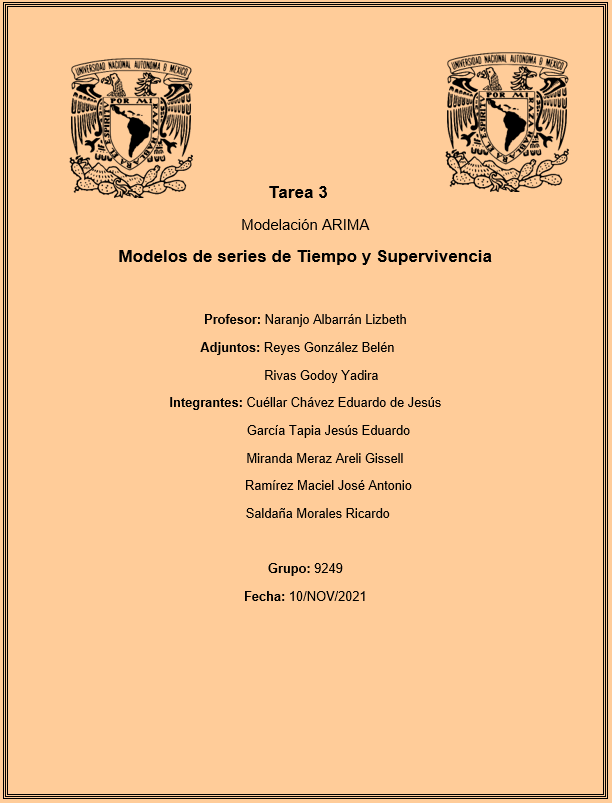
\includegraphics[width=2\linewidth]{CARATULA}

Analizar los datos Quarterly U.S. new plant/equip. expenditures 64 76
billions de la liberia tsdl de R.

\hypertarget{anuxe1lisis-descriptivo.}{%
\subsection{Análisis descriptivo.}\label{anuxe1lisis-descriptivo.}}

Grafique los datos, describa lo que observe (varianza constante o no
constante, descomposición clásica, tendencia, ciclos estacionales,
periodicidad de los ciclos).

Primero carguemos la librería tsdl, ya que los datos necesarios se
encuentran en dicha librería; así como otras necesarias para esta tarea.

\begin{Shaded}
\begin{Highlighting}[]
\FunctionTok{library}\NormalTok{(tsdl);}\FunctionTok{library}\NormalTok{(ggplot2);}\FunctionTok{library}\NormalTok{(itsmr);}\FunctionTok{library}\NormalTok{(forecast);}\FunctionTok{library}\NormalTok{(TSA);}\FunctionTok{library}\NormalTok{(lmtest)}
\FunctionTok{library}\NormalTok{(timeSeries);}\FunctionTok{library}\NormalTok{(timeSeries);}\FunctionTok{library}\NormalTok{(astsa);}
\FunctionTok{library}\NormalTok{(tseries);}\FunctionTok{library}\NormalTok{(forecast);}\FunctionTok{library}\NormalTok{(nortest);}\FunctionTok{library}\NormalTok{(dplyr);}\FunctionTok{library}\NormalTok{(imputeTS)}
\end{Highlighting}
\end{Shaded}

Cargamos la base de datos, nos aseguramos de que es la deseada.

\begin{Shaded}
\begin{Highlighting}[]
\NormalTok{Data }\OtherTok{\textless{}{-}}\NormalTok{ tsdl[[}\DecValTok{12}\NormalTok{]]}
\FunctionTok{attributes}\NormalTok{(Data)}
\end{Highlighting}
\end{Shaded}

\begin{verbatim}
## $tsp
## [1] 1964.00 1976.75    4.00
## 
## $class
## [1] "ts"
## 
## $source
## [1] "Abraham & Ledolter (1983)"
## 
## $description
## [1] "Quarterly U.S. new plant/equip. expenditures –64 – –76 billions"
## 
## $subject
## [1] "Microeconomic"
\end{verbatim}

Ahora que noa aseguramos de que es la base que queriamos, procedemos a
graficar:

\begin{Shaded}
\begin{Highlighting}[]
\FunctionTok{plot}\NormalTok{(Data, }\AttributeTok{main =} \StringTok{"Quarterly U.S. new plant/equip. expenditures }\SpecialCharTok{\textbackslash{}n}\StringTok{ 64 76 billions"}\NormalTok{)}
\end{Highlighting}
\end{Shaded}

\includegraphics{Tarea_3_files/figure-latex/unnamed-chunk-3-1.pdf}
\#\#\# Varianza Al menos de manera gráfica, la intuición nos dice que no
hay varianza constante, pero probémoslo con un test de homocedasticidad:

\begin{Shaded}
\begin{Highlighting}[]
\CommentTok{\#Los pasamos a series de tiempo}
\NormalTok{Serie}\OtherTok{\textless{}{-}}\FunctionTok{ts}\NormalTok{(}\AttributeTok{data=}\NormalTok{Data,}\AttributeTok{start=}\FunctionTok{c}\NormalTok{(}\DecValTok{1964}\NormalTok{,}\DecValTok{01}\NormalTok{),}\AttributeTok{end=}\FunctionTok{c}\NormalTok{(}\DecValTok{1976}\NormalTok{,}\DecValTok{4}\NormalTok{),}\AttributeTok{frequency=}\DecValTok{4}\NormalTok{)}
\NormalTok{tiempo}\OtherTok{\textless{}{-}}\FunctionTok{seq}\NormalTok{(}\DecValTok{1964}\SpecialCharTok{+}\DecValTok{0}\SpecialCharTok{/}\DecValTok{4}\NormalTok{, }\DecValTok{1976}\SpecialCharTok{+}\DecValTok{3}\SpecialCharTok{/}\DecValTok{4}\NormalTok{, }\AttributeTok{by =} \DecValTok{1}\SpecialCharTok{/}\DecValTok{4}\NormalTok{)}
\FunctionTok{bptest}\NormalTok{(Serie}\SpecialCharTok{\textasciitilde{}}\NormalTok{tiempo)}
\end{Highlighting}
\end{Shaded}

\begin{verbatim}
## 
##  studentized Breusch-Pagan test
## 
## data:  Serie ~ tiempo
## BP = 5.3713, df = 1, p-value = 0.02047
\end{verbatim}

Efectivamente, no pasa el test de homocedasticidad.

Veamos qué pasa si aplicamos la transformación logaritmo:

\begin{Shaded}
\begin{Highlighting}[]
\FunctionTok{bptest}\NormalTok{(}\FunctionTok{log}\NormalTok{(Serie)}\SpecialCharTok{\textasciitilde{}}\NormalTok{tiempo)}
\end{Highlighting}
\end{Shaded}

\begin{verbatim}
## 
##  studentized Breusch-Pagan test
## 
## data:  log(Serie) ~ tiempo
## BP = 1.965, df = 1, p-value = 0.161
\end{verbatim}

\begin{Shaded}
\begin{Highlighting}[]
\FunctionTok{plot}\NormalTok{(}\FunctionTok{log}\NormalTok{(Serie))}
\end{Highlighting}
\end{Shaded}

\includegraphics{Tarea_3_files/figure-latex/unnamed-chunk-5-1.pdf}
Tampoco ayudó, aunque mejoró un poco. Intentemos con la raíz cuadrada

\begin{Shaded}
\begin{Highlighting}[]
\FunctionTok{bptest}\NormalTok{(}\FunctionTok{sqrt}\NormalTok{(Serie)}\SpecialCharTok{\textasciitilde{}}\NormalTok{tiempo)}
\end{Highlighting}
\end{Shaded}

\begin{verbatim}
## 
##  studentized Breusch-Pagan test
## 
## data:  sqrt(Serie) ~ tiempo
## BP = 0.8651, df = 1, p-value = 0.3523
\end{verbatim}

\begin{Shaded}
\begin{Highlighting}[]
\FunctionTok{plot}\NormalTok{(}\FunctionTok{sqrt}\NormalTok{(Serie))}
\end{Highlighting}
\end{Shaded}

\includegraphics{Tarea_3_files/figure-latex/unnamed-chunk-6-1.pdf}
¡Logramos estabilizarla!

Veamos si es estacionaria.

\begin{Shaded}
\begin{Highlighting}[]
\FunctionTok{adf.test}\NormalTok{(}\FunctionTok{sqrt}\NormalTok{(Serie))}
\end{Highlighting}
\end{Shaded}

\begin{verbatim}
## 
##  Augmented Dickey-Fuller Test
## 
## data:  sqrt(Serie)
## Dickey-Fuller = -1.415, Lag order = 3, p-value = 0.8097
## alternative hypothesis: stationary
\end{verbatim}

\begin{Shaded}
\begin{Highlighting}[]
\FunctionTok{kpss.test}\NormalTok{(}\FunctionTok{sqrt}\NormalTok{(Serie))}
\end{Highlighting}
\end{Shaded}

\begin{verbatim}
## Warning in kpss.test(sqrt(Serie)): p-value smaller than printed p-value
\end{verbatim}

\begin{verbatim}
## 
##  KPSS Test for Level Stationarity
## 
## data:  sqrt(Serie)
## KPSS Level = 1.389, Truncation lag parameter = 3, p-value = 0.01
\end{verbatim}

\hypertarget{tendencia}{%
\subsubsection{Tendencia}\label{tendencia}}

Podemos observar una tendencia creciente que se presenta de manera
lineal (al parecer), de manera general a lo largo de la serie

\hypertarget{ciclos-estacionales}{%
\subsubsection{Ciclos estacionales}\label{ciclos-estacionales}}

Los ciclos están bastante marcados , y tiene sentido puesto que son los
datos de gastos de una empresa en maquinaria por trimestre, y en ese
contexto es lógico que se presenten ciclos: Generalmente decae del
último trimestre del año anterior al primero del año siguiente, para
después crecer en el segundo semestre, en el tercero se mantiene casi al
mismo nivel que el segundo, pero en el último aumenta; y es un
comportamiento que se repite año con año

\hypertarget{periodicidad-de-los-ciclos}{%
\subsubsection{Periodicidad de los
ciclos}\label{periodicidad-de-los-ciclos}}

Como comentamos en el apartado anterior, parece (al menos de manera
gráfica) que se tienen ciclos anuales.

\hypertarget{descomposiciuxf3n-cluxe1sica}{%
\subsubsection{Descomposición
clásica}\label{descomposiciuxf3n-cluxe1sica}}

Descomponeremos la serie por medio de filtros lineales:

\hypertarget{estabilizaciuxf3n-de-la-varianza}{%
\paragraph{Estabilización de la
varianza}\label{estabilizaciuxf3n-de-la-varianza}}

Aplicamos la transformación raíz cuadrada

\begin{Shaded}
\begin{Highlighting}[]
\NormalTok{Serie\_sq}\OtherTok{\textless{}{-}}\FunctionTok{sqrt}\NormalTok{(Serie)}
\FunctionTok{bptest}\NormalTok{(Serie\_sq}\SpecialCharTok{\textasciitilde{}}\NormalTok{tiempo)}
\end{Highlighting}
\end{Shaded}

\begin{verbatim}
## 
##  studentized Breusch-Pagan test
## 
## data:  Serie_sq ~ tiempo
## BP = 0.8651, df = 1, p-value = 0.3523
\end{verbatim}

Podemos asumir varianza constante

\hypertarget{periodicidad-de-ciclos}{%
\paragraph{Periodicidad de ciclos}\label{periodicidad-de-ciclos}}

\begin{Shaded}
\begin{Highlighting}[]
\CommentTok{\#Veamos la tendencia y los ciclos }
\NormalTok{Xt }\OtherTok{=}\NormalTok{ Serie\_sq}
\NormalTok{p }\OtherTok{=} \FunctionTok{periodogram}\NormalTok{(Xt, }\AttributeTok{main=}\StringTok{"Periodograma"}\NormalTok{, }\AttributeTok{col=}\DecValTok{4}\NormalTok{) }\CommentTok{\# Obtenemos el periodograma}
\end{Highlighting}
\end{Shaded}

\includegraphics{Tarea_3_files/figure-latex/unnamed-chunk-9-1.pdf}

\begin{Shaded}
\begin{Highlighting}[]
\FunctionTok{names}\NormalTok{(p)}
\end{Highlighting}
\end{Shaded}

\begin{verbatim}
##  [1] "freq"      "spec"      "coh"       "phase"     "kernel"    "df"       
##  [7] "bandwidth" "n.used"    "orig.n"    "series"    "snames"    "method"   
## [13] "taper"     "pad"       "detrend"   "demean"
\end{verbatim}

\begin{Shaded}
\begin{Highlighting}[]
\CommentTok{\# Ordenamos de mayor a menor las estimaciones del periodograma.}
\NormalTok{spec }\OtherTok{=} \FunctionTok{sort}\NormalTok{(p}\SpecialCharTok{$}\NormalTok{spec, }\AttributeTok{decreasing =} \ConstantTok{TRUE}\NormalTok{) }
\NormalTok{(}\AttributeTok{spec =}\NormalTok{ spec[}\DecValTok{1}\SpecialCharTok{:}\DecValTok{10}\NormalTok{]) }\CommentTok{\# Nos quedamos con los 8 coeficientes de mayor frecuencia.}
\end{Highlighting}
\end{Shaded}

\begin{verbatim}
##  [1] 12.9646281  4.2701894  1.3676068  1.1581310  1.0460373  0.4486585
##  [7]  0.4395386  0.3466661  0.2593484  0.1970454
\end{verbatim}

\begin{Shaded}
\begin{Highlighting}[]
\NormalTok{i }\OtherTok{=} \FunctionTok{match}\NormalTok{(spec, p}\SpecialCharTok{$}\NormalTok{spec) }\CommentTok{\# Buscamos sus indices en el periodograma.}
\NormalTok{d }\OtherTok{=}\NormalTok{ p}\SpecialCharTok{$}\NormalTok{freq }\CommentTok{\# Vemos las frecuencias del periodograma.}
\NormalTok{d }\OtherTok{=}\NormalTok{ d[i] }\CommentTok{\# Nos quedamos con las frecuencias que nos interesan.}

\FunctionTok{cbind}\NormalTok{(spec,d,i)}\CommentTok{\#}
\end{Highlighting}
\end{Shaded}

\begin{verbatim}
##             spec          d  i
##  [1,] 12.9646281 0.01851852  1
##  [2,]  4.2701894 0.03703704  2
##  [3,]  1.3676068 0.05555556  3
##  [4,]  1.1581310 0.50000000 27
##  [5,]  1.0460373 0.07407407  4
##  [6,]  0.4486585 0.11111111  6
##  [7,]  0.4395386 0.09259259  5
##  [8,]  0.3466661 0.24074074 13
##  [9,]  0.2593484 0.12962963  7
## [10,]  0.1970454 0.14814815  8
\end{verbatim}

\begin{Shaded}
\begin{Highlighting}[]
\NormalTok{d }\OtherTok{=} \DecValTok{1} \SpecialCharTok{/}\NormalTok{ d }\CommentTok{\# Obtenemos los parametros para utilizar en promedios moviles.}
\NormalTok{d }\OtherTok{=} \FunctionTok{floor}\NormalTok{(d) }\CommentTok{\#}
\NormalTok{(}\AttributeTok{d =} \FunctionTok{sort}\NormalTok{(d))}
\end{Highlighting}
\end{Shaded}

\begin{verbatim}
##  [1]  2  4  6  7  9 10 13 18 27 54
\end{verbatim}

\begin{Shaded}
\begin{Highlighting}[]
\CommentTok{\# Quitamos los periodos mas grandes}
\NormalTok{d }\OtherTok{=}\NormalTok{ d[}\SpecialCharTok{{-}}\FunctionTok{length}\NormalTok{(d)] }
\NormalTok{d }\OtherTok{=}\NormalTok{ d[}\SpecialCharTok{{-}}\FunctionTok{length}\NormalTok{(d)]}
\CommentTok{\# Quitamos el más pequeño}
\NormalTok{d }\OtherTok{=}\NormalTok{ d[}\SpecialCharTok{{-}}\DecValTok{1}\NormalTok{]}
\NormalTok{d }\CommentTok{\#Posibles periodos del ciclo }
\end{Highlighting}
\end{Shaded}

\begin{verbatim}
## [1]  4  6  7  9 10 13 18
\end{verbatim}

\begin{Shaded}
\begin{Highlighting}[]
\CommentTok{\#Realizamos la grafica:}
\NormalTok{col }\OtherTok{=} \FunctionTok{c}\NormalTok{(}\StringTok{"dodgerblue1"}\NormalTok{, }\StringTok{"darkorange1"}\NormalTok{, }\StringTok{"brown"}\NormalTok{)}
\FunctionTok{plot}\NormalTok{(Serie\_sq, }\AttributeTok{lwd =} \DecValTok{3}\NormalTok{, }\AttributeTok{xlab =} \StringTok{"Tiempo"}\NormalTok{, }\AttributeTok{col =} \StringTok{"gray0"}\NormalTok{,}
     \AttributeTok{main =} \StringTok{"Serie con varianza Homocedastica"}\NormalTok{,}
     \AttributeTok{ylab =} \StringTok{"Numero"}\NormalTok{, }\AttributeTok{col.main =} \StringTok{"burlywood"}\NormalTok{)}
\ControlFlowTok{for}\NormalTok{ (i }\ControlFlowTok{in} \DecValTok{1}\SpecialCharTok{:}\DecValTok{3}\NormalTok{) \{}
  \FunctionTok{lines}\NormalTok{(tiempo, stats}\SpecialCharTok{::}\FunctionTok{filter}\NormalTok{(Serie\_sq, }\FunctionTok{rep}\NormalTok{(}\DecValTok{1} \SpecialCharTok{/}\NormalTok{ d[i], d[i])), }\AttributeTok{col =}\NormalTok{ col[i], }
        \AttributeTok{lwd =} \DecValTok{3}\NormalTok{)}
\NormalTok{\}}
\FunctionTok{legend}\NormalTok{(}\StringTok{"bottomright"}\NormalTok{, }\AttributeTok{col =}\NormalTok{ col, }\AttributeTok{lty =} \DecValTok{2}\NormalTok{, }\AttributeTok{lwd =} \DecValTok{2}\NormalTok{, }\AttributeTok{bty =} \StringTok{"n"}\NormalTok{,}
       \AttributeTok{legend =} \FunctionTok{c}\NormalTok{(}\FunctionTok{paste}\NormalTok{(}\StringTok{"d = "}\NormalTok{, d[}\DecValTok{1}\NormalTok{]), }\FunctionTok{paste}\NormalTok{(}\StringTok{"d = "}\NormalTok{, d[}\DecValTok{2}\NormalTok{]),}
                  \FunctionTok{paste}\NormalTok{(}\StringTok{"d = "}\NormalTok{, d[}\DecValTok{3}\NormalTok{])), }\AttributeTok{cex =} \DecValTok{1}\NormalTok{)}
\end{Highlighting}
\end{Shaded}

\includegraphics{Tarea_3_files/figure-latex/unnamed-chunk-9-2.pdf}
Notemos que \(d=2\) parece sobreajustar un poco nuestra gráfica, de
hecho, bastante. Sin embargo, con \(d=4\) podemos obtener un buen
suavizamiento sin pagar el costo de otros \(2\) datos al elegir \(d=6\).
Veamos el ACF y PACF:

\begin{Shaded}
\begin{Highlighting}[]
\FunctionTok{tsdisplay}\NormalTok{(Serie\_sq)}
\end{Highlighting}
\end{Shaded}

\includegraphics{Tarea_3_files/figure-latex/unnamed-chunk-10-1.pdf} Y,
junto con este último resultado, nos parece ideal concluir que el ciclo
es \(d=4\)

\hypertarget{tendencia-1}{%
\subsubsection{Tendencia}\label{tendencia-1}}

Ahora, aislemos la tendencia:

\begin{Shaded}
\begin{Highlighting}[]
\NormalTok{tendencia }\OtherTok{=}\NormalTok{ stats}\SpecialCharTok{::}\FunctionTok{filter}\NormalTok{(Serie\_sq, }\FunctionTok{rep}\NormalTok{(}\DecValTok{1}\SpecialCharTok{/}\DecValTok{4}\NormalTok{, }\DecValTok{4}\NormalTok{))}
\FunctionTok{plot}\NormalTok{(Serie\_sq, }\AttributeTok{lwd =} \DecValTok{3}\NormalTok{, }\AttributeTok{xlab =} \StringTok{"Tiempo"}\NormalTok{, }\AttributeTok{col =} \StringTok{"black"}\NormalTok{,}
     \AttributeTok{main =} \StringTok{"Tendencia"}\NormalTok{,}
     \AttributeTok{ylab =} \StringTok{"Numero"}\NormalTok{, }\AttributeTok{col.main =} \StringTok{"burlywood"}\NormalTok{)}
\FunctionTok{lines}\NormalTok{(tendencia, }\AttributeTok{col =} \StringTok{"gold4"}\NormalTok{, }\AttributeTok{lwd =} \DecValTok{4}\NormalTok{)}
\FunctionTok{legend}\NormalTok{(}\StringTok{"bottomright"}\NormalTok{, }\AttributeTok{col =} \StringTok{"gold4"}\NormalTok{, }\AttributeTok{lty =} \DecValTok{1}\NormalTok{, }\AttributeTok{lwd =} \DecValTok{2}\NormalTok{, }\AttributeTok{bty =} \StringTok{"n"}\NormalTok{,}
       \AttributeTok{legend =} \StringTok{"Tendencia"}\NormalTok{, }\AttributeTok{cex =} \DecValTok{1}\NormalTok{)}
\end{Highlighting}
\end{Shaded}

\includegraphics{Tarea_3_files/figure-latex/unnamed-chunk-11-1.pdf}

Lo que refuerza lo que creíamos: Tiene tebdebcua creciente casi de
manera general.

\hypertarget{tendencia-2}{%
\paragraph{Tendencia}\label{tendencia-2}}

\begin{Shaded}
\begin{Highlighting}[]
\CommentTok{\# Quitamos la tendencia}
\CommentTok{\# Solo trabajamos con la serie cuya varianza es cte. }

\NormalTok{datosSinTendencia }\OtherTok{=}\NormalTok{ Serie\_sq }\SpecialCharTok{{-}}\NormalTok{ tendencia }\CommentTok{\# Serie sin tendencia}
\FunctionTok{plot}\NormalTok{(datosSinTendencia, }\AttributeTok{main=}\StringTok{"Serie sin tendencia"}\NormalTok{, }\AttributeTok{lwd=}\DecValTok{2}\NormalTok{, }\AttributeTok{ylab=}\StringTok{""}\NormalTok{, }\AttributeTok{col=}\DecValTok{14}\NormalTok{)}
\end{Highlighting}
\end{Shaded}

\includegraphics{Tarea_3_files/figure-latex/unnamed-chunk-12-1.pdf}

\begin{Shaded}
\begin{Highlighting}[]
\CommentTok{\# Convertimos datosSinTendencia en objeto TS, dado que hicimos promedios moviles}

\NormalTok{inicio}\OtherTok{=}\FunctionTok{start}\NormalTok{(Serie\_sq)}
\NormalTok{final}\OtherTok{=}\FunctionTok{end}\NormalTok{(Serie\_sq)}

\NormalTok{datos.ts4}\OtherTok{=}\FunctionTok{ts}\NormalTok{(datosSinTendencia, }\AttributeTok{frequency =} \DecValTok{4}\NormalTok{, }\AttributeTok{start=}\NormalTok{inicio,}\AttributeTok{end=}\NormalTok{final) }
\FunctionTok{which}\NormalTok{(}\FunctionTok{is.na}\NormalTok{(datos.ts4)}\SpecialCharTok{==}\NormalTok{T)}
\end{Highlighting}
\end{Shaded}

\begin{verbatim}
## [1]  1 51 52
\end{verbatim}

\begin{Shaded}
\begin{Highlighting}[]
\FunctionTok{par}\NormalTok{(}\AttributeTok{mfrow =} \FunctionTok{c}\NormalTok{(}\DecValTok{3}\NormalTok{,}\DecValTok{1}\NormalTok{))}
\FunctionTok{plot}\NormalTok{(datos.ts4, }\AttributeTok{col =} \StringTok{"slateblue4"}\NormalTok{, }\AttributeTok{lwd =} \DecValTok{2}\NormalTok{, }\AttributeTok{ylab =} \StringTok{" "}\NormalTok{, }\AttributeTok{type =} \StringTok{"l"}\NormalTok{,}
     \AttributeTok{main =} \StringTok{"Serie de tiempo sin tendencia"}\NormalTok{, }\AttributeTok{xlab =} \StringTok{"Tiempo"}\NormalTok{)}

\FunctionTok{acf}\NormalTok{(datos.ts4[}\DecValTok{2}\SpecialCharTok{:}\DecValTok{50}\NormalTok{])}
\FunctionTok{pacf}\NormalTok{(datos.ts4[}\DecValTok{2}\SpecialCharTok{:}\DecValTok{50}\NormalTok{])}
\end{Highlighting}
\end{Shaded}

\includegraphics{Tarea_3_files/figure-latex/unnamed-chunk-12-2.pdf}

\begin{Shaded}
\begin{Highlighting}[]
\FunctionTok{par}\NormalTok{(}\AttributeTok{mfrow =} \FunctionTok{c}\NormalTok{(}\DecValTok{1}\NormalTok{,}\DecValTok{1}\NormalTok{))}
\FunctionTok{tsdisplay}\NormalTok{(datos.ts4, }\AttributeTok{col=}\StringTok{"purple"}\NormalTok{, }\AttributeTok{lwd=}\DecValTok{2}\NormalTok{)}
\end{Highlighting}
\end{Shaded}

\includegraphics{Tarea_3_files/figure-latex/unnamed-chunk-12-3.pdf}
Parece que eliminamos la tendencia, ahora tratemos de verificar los
ciclos

\#Ciclos o parte estacional Ahora, estimaremos la parte estacional.
Tenemos que d = 4. Originalmente contábamos con 52 datos, pero ahora
tenemos 48 (por los NA), entonces \(\frac{48}{4}=12\) ciclos.

\begin{Shaded}
\begin{Highlighting}[]
\CommentTok{\# Creamos un ciclo promedio que estime la parte estacional,}
\CommentTok{\# usando la serie sin tendencia.}
\NormalTok{d }\OtherTok{=} \DecValTok{4}
\NormalTok{k }\OtherTok{=} \FunctionTok{length}\NormalTok{(datos.ts4) }\SpecialCharTok{/}\NormalTok{ d }\CommentTok{\# Numero de ciclos de la serie sin tendencia}
\NormalTok{w }\OtherTok{=} \FunctionTok{rep}\NormalTok{(}\DecValTok{0}\NormalTok{, }\DecValTok{4}\NormalTok{) }
\CommentTok{\# Para el resto de los trimestres}
\ControlFlowTok{for}\NormalTok{ (i }\ControlFlowTok{in} \DecValTok{1}\SpecialCharTok{:}\DecValTok{4}\NormalTok{)}
\NormalTok{  w[i] }\OtherTok{=} \FunctionTok{sum}\NormalTok{(datos.ts4[d }\SpecialCharTok{*}\NormalTok{ (}\DecValTok{0}\SpecialCharTok{:}\NormalTok{(k}\DecValTok{{-}1}\NormalTok{)) }\SpecialCharTok{+}\NormalTok{ i], }\AttributeTok{na.rm =} \ConstantTok{TRUE}\NormalTok{) }\SpecialCharTok{/}\NormalTok{ k}

\CommentTok{\# Ahora, ajustamos el ciclo obtenido}
\NormalTok{ciclo  }\OtherTok{=}\NormalTok{ w }\SpecialCharTok{{-}} \FunctionTok{mean}\NormalTok{(w)}
\NormalTok{ciclo }\OtherTok{=} \FunctionTok{ts}\NormalTok{(}\FunctionTok{rep}\NormalTok{(ciclo, }\AttributeTok{times =}\NormalTok{ k), }\AttributeTok{start =} \FunctionTok{start}\NormalTok{(Serie\_sq), }
           \AttributeTok{frequency =} \FunctionTok{frequency}\NormalTok{(Serie\_sq))}
\FunctionTok{par}\NormalTok{(}\AttributeTok{mfrow =} \FunctionTok{c}\NormalTok{(}\DecValTok{1}\NormalTok{, }\DecValTok{1}\NormalTok{))}
\FunctionTok{plot}\NormalTok{(ciclo, }\AttributeTok{col =}\DecValTok{20}\NormalTok{, }\AttributeTok{lwd =} \DecValTok{3}\NormalTok{, }\AttributeTok{ylab =} \StringTok{" "}\NormalTok{, }\AttributeTok{xlab =} \StringTok{"Tiempo"}\NormalTok{,}
     \AttributeTok{main =} \StringTok{"Ciclos de la serie"}\NormalTok{)}\CommentTok{\# Es el ciclo de la serie }
\end{Highlighting}
\end{Shaded}

\includegraphics{Tarea_3_files/figure-latex/unnamed-chunk-13-1.pdf}

\begin{Shaded}
\begin{Highlighting}[]
\CommentTok{\# Ciclos anuales}
\end{Highlighting}
\end{Shaded}

Ahora verifiquemos de manera gráfica

\begin{Shaded}
\begin{Highlighting}[]
\CommentTok{\# Calculamos la parte aleatoria}
\NormalTok{parte\_aleatoria }\OtherTok{=}\NormalTok{ datos.ts4 }\SpecialCharTok{{-}}\NormalTok{ ciclo}
\FunctionTok{plot}\NormalTok{(parte\_aleatoria, }\AttributeTok{main =} \StringTok{"Parte aleatoria"}\NormalTok{, }
     \AttributeTok{col =}\DecValTok{30}\NormalTok{, }\AttributeTok{lwd =} \DecValTok{3}\NormalTok{, }\AttributeTok{xlab =} \StringTok{"Tiempo"}\NormalTok{, }\AttributeTok{ylab =} \StringTok{""}\NormalTok{) }
\end{Highlighting}
\end{Shaded}

\includegraphics{Tarea_3_files/figure-latex/unnamed-chunk-14-1.pdf}

\begin{Shaded}
\begin{Highlighting}[]
\FunctionTok{plot}\NormalTok{(Serie\_sq)}
\end{Highlighting}
\end{Shaded}

\includegraphics{Tarea_3_files/figure-latex/unnamed-chunk-14-2.pdf}

\begin{Shaded}
\begin{Highlighting}[]
\CommentTok{\# Con esto, ya tenemos nuestras series}

\NormalTok{componentes }\OtherTok{=}\NormalTok{ tendencia }\SpecialCharTok{+}\NormalTok{ ciclo}\SpecialCharTok{+}\NormalTok{parte\_aleatoria}
\NormalTok{componentes }\OtherTok{=} \FunctionTok{ts}\NormalTok{(componentes, }\AttributeTok{start =} \FunctionTok{start}\NormalTok{(Serie\_sq), }\AttributeTok{frequency =} \DecValTok{4}\NormalTok{)}
\FunctionTok{par}\NormalTok{(}\AttributeTok{mfrow =} \FunctionTok{c}\NormalTok{(}\DecValTok{2}\NormalTok{,}\DecValTok{1}\NormalTok{))}
\FunctionTok{plot}\NormalTok{(Serie\_sq, }\AttributeTok{col=}\DecValTok{28}\NormalTok{, }\AttributeTok{las=}\DecValTok{1}\NormalTok{, }\AttributeTok{main=}\StringTok{"Serie con varianza constante"}\NormalTok{, }\AttributeTok{lwd=}\DecValTok{3}\NormalTok{, }\AttributeTok{xlab=}\StringTok{""}\NormalTok{,}\AttributeTok{ylab=}\StringTok{""}\NormalTok{)}
\FunctionTok{plot}\NormalTok{(componentes, }\AttributeTok{col =} \DecValTok{18}\NormalTok{, }\AttributeTok{lwd =} \DecValTok{3}\NormalTok{, }\AttributeTok{las=}\DecValTok{1}\NormalTok{, }\AttributeTok{main=}\StringTok{"Yt=tendencia+ciclos+aleatoria"}\NormalTok{, }\AttributeTok{xlab=}\StringTok{""}\NormalTok{,}\AttributeTok{ylab=}\StringTok{""}\NormalTok{)}
\end{Highlighting}
\end{Shaded}

\includegraphics{Tarea_3_files/figure-latex/unnamed-chunk-14-3.pdf}

\begin{Shaded}
\begin{Highlighting}[]
\FunctionTok{par}\NormalTok{(}\AttributeTok{mfrow =} \FunctionTok{c}\NormalTok{(}\DecValTok{1}\NormalTok{,}\DecValTok{1}\NormalTok{))}
\FunctionTok{plot}\NormalTok{(Serie\_sq,}\AttributeTok{col=}\StringTok{"darkblue"}\NormalTok{, }\AttributeTok{las=}\DecValTok{1}\NormalTok{, }\AttributeTok{lwd=}\DecValTok{3}\NormalTok{,}\AttributeTok{main=}\StringTok{"Serie\_ln"}\NormalTok{, }\AttributeTok{ylab=}\StringTok{""}\NormalTok{,}\AttributeTok{xlab=}\StringTok{""}\NormalTok{)}
\FunctionTok{invisible}\NormalTok{(}\FunctionTok{lines}\NormalTok{(componentes, }\AttributeTok{type=}\StringTok{"l"}\NormalTok{, }\AttributeTok{lwd=}\DecValTok{3}\NormalTok{, }\AttributeTok{col=}\StringTok{"green"}\NormalTok{,}\AttributeTok{lty=}\DecValTok{6}\NormalTok{))}
\FunctionTok{legend}\NormalTok{(}\StringTok{"bottomright"}\NormalTok{, }\AttributeTok{col =} \FunctionTok{c}\NormalTok{(}\StringTok{"darkblue"}\NormalTok{,}\StringTok{"green"}\NormalTok{), }\AttributeTok{lty =} \DecValTok{1}\NormalTok{, }\AttributeTok{lwd =} \DecValTok{2}\NormalTok{, }\AttributeTok{bty =} \StringTok{"n"}\NormalTok{,}
       \AttributeTok{legend =} \FunctionTok{c}\NormalTok{(}\StringTok{"Serie Homocedastica"}\NormalTok{,}\StringTok{"Yt=T+C+A"}\NormalTok{), }\AttributeTok{cex =} \DecValTok{1}\NormalTok{)}
\end{Highlighting}
\end{Shaded}

\includegraphics{Tarea_3_files/figure-latex/unnamed-chunk-14-4.pdf}

¡Logramos identificar los componentes de la serie!

\hypertarget{missing-data}{%
\subsection{Missing data}\label{missing-data}}

Suponga que las observaciones de 1971 Qtr1, 1973 Qtr2 y 1973 Qtr3, son
datos faltantes NA, es decir, sustituya estas observaciones por NA.

Use al menos dos métodos de imputación de la paqueteríaa imputeTS. ¿Cuál
método es adecuado para estos datos? (Note que el valor imputado debe
aproximarse al valor omitido).

Vamos a poner los datos que se piden, como NA:

\begin{Shaded}
\begin{Highlighting}[]
\NormalTok{Original}\OtherTok{=}\NormalTok{Serie[}\DecValTok{29}\NormalTok{]}
\NormalTok{Original[}\DecValTok{2}\NormalTok{]}\OtherTok{=}\NormalTok{Serie[}\DecValTok{38}\NormalTok{]}
\NormalTok{Original[}\DecValTok{3}\NormalTok{]}\OtherTok{=}\NormalTok{Serie[}\DecValTok{39}\NormalTok{]}
\NormalTok{Serie\_2}\OtherTok{=}\NormalTok{Serie}
\NormalTok{Serie\_2[}\DecValTok{29}\NormalTok{]}\OtherTok{=}\ConstantTok{NA}
\NormalTok{Serie\_2[}\DecValTok{38}\SpecialCharTok{:}\DecValTok{39}\NormalTok{]}\OtherTok{=}\ConstantTok{NA}
\NormalTok{Serie\_2}
\end{Highlighting}
\end{Shaded}

\begin{verbatim}
##       Qtr1  Qtr2  Qtr3  Qtr4
## 1964 10.00 11.85 11.70 13.42
## 1965 11.20 13.63 13.65 15.93
## 1966 13.33 16.05 15.92 18.22
## 1967 14.46 16.69 16.20 18.12
## 1968 15.10 16.85 16.79 19.03
## 1969 16.04 18.81 19.25 21.46
## 1970 17.47 20.33 20.26 21.66
## 1971    NA 20.60 20.14 22.79
## 1972 19.38 22.01 21.86 25.20
## 1973 21.50    NA    NA 28.48
## 1974 24.10 28.16 28.23 31.92
## 1975 25.82 28.43 27.79 30.74
## 1976 25.87 29.70 30.41 34.52
\end{verbatim}

Ahora, veamos método por método:

Un vistazo a la documentación de la paquetería mencionada nos menciona
los siguientes métodos:

\begin{enumerate}
\item na\_interpolation:

Missing Value Imputation by Interpolation. Acepta 3 tipos:
\begin{enumerate}
\item "linear" - for linear interpolation using approx (default choice)


```r
Comparaciones=data.frame(Original)
na_interpolation_lineal=na_interpolation(Serie_2,option='linear')[29]-Original[1]
na_interpolation_lineal[2:3]=na_interpolation(Serie_2,option='linear')[38:39]-Original[2:3]
Comparaciones['na_interpolation_lineal']=na_interpolation_lineal
Comparaciones
```

```
##   Original na_interpolation_lineal
## 1    17.68               3.4500000
## 2    24.73              -0.9033333
## 3    25.04               1.1133333
```

\item "spline" - for spline interpolation using spline

```r
na_interpolation(Serie_2,option='spline')
```

```
##          Qtr1     Qtr2     Qtr3     Qtr4
## 1964 10.00000 11.85000 11.70000 13.42000
## 1965 11.20000 13.63000 13.65000 15.93000
## 1966 13.33000 16.05000 15.92000 18.22000
## 1967 14.46000 16.69000 16.20000 18.12000
## 1968 15.10000 16.85000 16.79000 19.03000
## 1969 16.04000 18.81000 19.25000 21.46000
## 1970 17.47000 20.33000 20.26000 21.66000
## 1971 21.91352 20.60000 20.14000 22.79000
## 1972 19.38000 22.01000 21.86000 25.20000
## 1973 21.50000 22.89979 27.71251 28.48000
## 1974 24.10000 28.16000 28.23000 31.92000
## 1975 25.82000 28.43000 27.79000 30.74000
## 1976 25.87000 29.70000 30.41000 34.52000
```

\item "stine" - for Stineman interpolation using stinterp

```r
na_interpolation(Serie_2,option='stine')
```

```
##          Qtr1     Qtr2     Qtr3     Qtr4
## 1964 10.00000 11.85000 11.70000 13.42000
## 1965 11.20000 13.63000 13.65000 15.93000
## 1966 13.33000 16.05000 15.92000 18.22000
## 1967 14.46000 16.69000 16.20000 18.12000
## 1968 15.10000 16.85000 16.79000 19.03000
## 1969 16.04000 18.81000 19.25000 21.46000
## 1970 17.47000 20.33000 20.26000 21.66000
## 1971 21.13000 20.60000 20.14000 22.79000
## 1972 19.38000 22.01000 21.86000 25.20000
## 1973 21.50000 23.10575 26.86069 28.48000
## 1974 24.10000 28.16000 28.23000 31.92000
## 1975 25.82000 28.43000 27.79000 30.74000
## 1976 25.87000 29.70000 30.41000 34.52000
```

\end{enumerate}

\item

na\_kalman:

Missing Value Imputation by Kalman Smoothing and State Space Models.
Acepta los suientes modelos:

\begin{enumerate}
\item "auto.arima" - For using the state space representation of arima model (using auto.arima) (default choice)

```r
na_kalman(Serie_2,model='auto.arima')
```

```
##          Qtr1     Qtr2     Qtr3     Qtr4
## 1964 10.00000 11.85000 11.70000 13.42000
## 1965 11.20000 13.63000 13.65000 15.93000
## 1966 13.33000 16.05000 15.92000 18.22000
## 1967 14.46000 16.69000 16.20000 18.12000
## 1968 15.10000 16.85000 16.79000 19.03000
## 1969 16.04000 18.81000 19.25000 21.46000
## 1970 17.47000 20.33000 20.26000 21.66000
## 1971 17.88402 20.60000 20.14000 22.79000
## 1972 19.38000 22.01000 21.86000 25.20000
## 1973 21.50000 24.99381 25.24268 28.48000
## 1974 24.10000 28.16000 28.23000 31.92000
## 1975 25.82000 28.43000 27.79000 30.74000
## 1976 25.87000 29.70000 30.41000 34.52000
```

\item "StructTS" - For using a structural model fitted by maximum likelihood (using StructTS)

```r
na_kalman(Serie_2,model='StructTS')
```

```
##          Qtr1     Qtr2     Qtr3     Qtr4
## 1964 10.00000 11.85000 11.70000 13.42000
## 1965 11.20000 13.63000 13.65000 15.93000
## 1966 13.33000 16.05000 15.92000 18.22000
## 1967 14.46000 16.69000 16.20000 18.12000
## 1968 15.10000 16.85000 16.79000 19.03000
## 1969 16.04000 18.81000 19.25000 21.46000
## 1970 17.47000 20.33000 20.26000 21.66000
## 1971 17.98114 20.60000 20.14000 22.79000
## 1972 19.38000 22.01000 21.86000 25.20000
## 1973 21.50000 24.82428 24.92793 28.48000
## 1974 24.10000 28.16000 28.23000 31.92000
## 1975 25.82000 28.43000 27.79000 30.74000
## 1976 25.87000 29.70000 30.41000 34.52000
```
\end{enumerate}
\item

na\_locf:

Missing Value Imputation by Last Observation Carried Forward. Acepta los
siguientes métodos:

\begin{enumerate}

\item "locf" - for Last Observation Carried Forward (default choice)

```r
na_locf(Serie_2,option = 'locf')
```

```
##       Qtr1  Qtr2  Qtr3  Qtr4
## 1964 10.00 11.85 11.70 13.42
## 1965 11.20 13.63 13.65 15.93
## 1966 13.33 16.05 15.92 18.22
## 1967 14.46 16.69 16.20 18.12
## 1968 15.10 16.85 16.79 19.03
## 1969 16.04 18.81 19.25 21.46
## 1970 17.47 20.33 20.26 21.66
## 1971 21.66 20.60 20.14 22.79
## 1972 19.38 22.01 21.86 25.20
## 1973 21.50 21.50 21.50 28.48
## 1974 24.10 28.16 28.23 31.92
## 1975 25.82 28.43 27.79 30.74
## 1976 25.87 29.70 30.41 34.52
```

\item "nocb" - for Next Observation Carried Backward

```r
na_locf(Serie_2,option = 'nocb')
```

```
##       Qtr1  Qtr2  Qtr3  Qtr4
## 1964 10.00 11.85 11.70 13.42
## 1965 11.20 13.63 13.65 15.93
## 1966 13.33 16.05 15.92 18.22
## 1967 14.46 16.69 16.20 18.12
## 1968 15.10 16.85 16.79 19.03
## 1969 16.04 18.81 19.25 21.46
## 1970 17.47 20.33 20.26 21.66
## 1971 20.60 20.60 20.14 22.79
## 1972 19.38 22.01 21.86 25.20
## 1973 21.50 28.48 28.48 28.48
## 1974 24.10 28.16 28.23 31.92
## 1975 25.82 28.43 27.79 30.74
## 1976 25.87 29.70 30.41 34.52
```

\end{enumerate}

\item

na\_ma Missing:

Value Imputation by Weighted Moving Average. Acepta los siguientes
métodos:

\begin{enumerate}
\item "simple" - Simple Moving Average (SMA)

```r
na_ma(Serie_2,weighting = 'simple')
```

```
##          Qtr1     Qtr2     Qtr3     Qtr4
## 1964 10.00000 11.85000 11.70000 13.42000
## 1965 11.20000 13.63000 13.65000 15.93000
## 1966 13.33000 16.05000 15.92000 18.22000
## 1967 14.46000 16.69000 16.20000 18.12000
## 1968 15.10000 16.85000 16.79000 19.03000
## 1969 16.04000 18.81000 19.25000 21.46000
## 1970 17.47000 20.33000 20.26000 21.66000
## 1971 20.32875 20.60000 20.14000 22.79000
## 1972 19.38000 22.01000 21.86000 25.20000
## 1973 21.50000 24.47286 25.36143 28.48000
## 1974 24.10000 28.16000 28.23000 31.92000
## 1975 25.82000 28.43000 27.79000 30.74000
## 1976 25.87000 29.70000 30.41000 34.52000
```

\item "linear" - Linear Weighted Moving Average (LWMA)

```r
na_ma(Serie_2,weighting = 'linear')
```

```
##          Qtr1     Qtr2     Qtr3     Qtr4
## 1964 10.00000 11.85000 11.70000 13.42000
## 1965 11.20000 13.63000 13.65000 15.93000
## 1966 13.33000 16.05000 15.92000 18.22000
## 1967 14.46000 16.69000 16.20000 18.12000
## 1968 15.10000 16.85000 16.79000 19.03000
## 1969 16.04000 18.81000 19.25000 21.46000
## 1970 17.47000 20.33000 20.26000 21.66000
## 1971 20.55065 20.60000 20.14000 22.79000
## 1972 19.38000 22.01000 21.86000 25.20000
## 1973 21.50000 24.27452 25.54742 28.48000
## 1974 24.10000 28.16000 28.23000 31.92000
## 1975 25.82000 28.43000 27.79000 30.74000
## 1976 25.87000 29.70000 30.41000 34.52000
```
\item "exponential" - Exponential Weighted Moving Average (EWMA) (default choice)

```r
na_ma(Serie_2,weighting = 'exponential')
```

```
##          Qtr1     Qtr2     Qtr3     Qtr4
## 1964 10.00000 11.85000 11.70000 13.42000
## 1965 11.20000 13.63000 13.65000 15.93000
## 1966 13.33000 16.05000 15.92000 18.22000
## 1967 14.46000 16.69000 16.20000 18.12000
## 1968 15.10000 16.85000 16.79000 19.03000
## 1969 16.04000 18.81000 19.25000 21.46000
## 1970 17.47000 20.33000 20.26000 21.66000
## 1971 20.75900 20.60000 20.14000 22.79000
## 1972 19.38000 22.01000 21.86000 25.20000
## 1973 21.50000 24.03682 25.77500 28.48000
## 1974 24.10000 28.16000 28.23000 31.92000
## 1975 25.82000 28.43000 27.79000 30.74000
## 1976 25.87000 29.70000 30.41000 34.52000
```
\end{enumerate}

\item

na\_mean Missing:

Value Imputation by Mean Value. Acepta los siguientes métodos:

\begin{enumerate}
\item "mean" - take the mean for imputation (default choice)

```r
na_mean(Serie_2,option = 'mean')
```

```
##       Qtr1  Qtr2  Qtr3  Qtr4
## 1964 10.00 11.85 11.70 13.42
## 1965 11.20 13.63 13.65 15.93
## 1966 13.33 16.05 15.92 18.22
## 1967 14.46 16.69 16.20 18.12
## 1968 15.10 16.85 16.79 19.03
## 1969 16.04 18.81 19.25 21.46
## 1970 17.47 20.33 20.26 21.66
## 1971 20.43 20.60 20.14 22.79
## 1972 19.38 22.01 21.86 25.20
## 1973 21.50 20.43 20.43 28.48
## 1974 24.10 28.16 28.23 31.92
## 1975 25.82 28.43 27.79 30.74
## 1976 25.87 29.70 30.41 34.52
```
\item "median" - take the median for imputation

```r
na_mean(Serie_2,option = 'median')
```

```
##       Qtr1  Qtr2  Qtr3  Qtr4
## 1964 10.00 11.85 11.70 13.42
## 1965 11.20 13.63 13.65 15.93
## 1966 13.33 16.05 15.92 18.22
## 1967 14.46 16.69 16.20 18.12
## 1968 15.10 16.85 16.79 19.03
## 1969 16.04 18.81 19.25 21.46
## 1970 17.47 20.33 20.26 21.66
## 1971 19.38 20.60 20.14 22.79
## 1972 19.38 22.01 21.86 25.20
## 1973 21.50 19.38 19.38 28.48
## 1974 24.10 28.16 28.23 31.92
## 1975 25.82 28.43 27.79 30.74
## 1976 25.87 29.70 30.41 34.52
```
\item "mode" - take the mode for imputation

```r
na_mean(Serie_2,option = 'mode')
```

```
##       Qtr1  Qtr2  Qtr3  Qtr4
## 1964 10.00 11.85 11.70 13.42
## 1965 11.20 13.63 13.65 15.93
## 1966 13.33 16.05 15.92 18.22
## 1967 14.46 16.69 16.20 18.12
## 1968 15.10 16.85 16.79 19.03
## 1969 16.04 18.81 19.25 21.46
## 1970 17.47 20.33 20.26 21.66
## 1971 10.00 20.60 20.14 22.79
## 1972 19.38 22.01 21.86 25.20
## 1973 21.50 10.00 10.00 28.48
## 1974 24.10 28.16 28.23 31.92
## 1975 25.82 28.43 27.79 30.74
## 1976 25.87 29.70 30.41 34.52
```
\item "harmonic" - take the harmonic mean

```r
na_mean(Serie_2,option = 'harmonic')
```

```
##          Qtr1     Qtr2     Qtr3     Qtr4
## 1964 10.00000 11.85000 11.70000 13.42000
## 1965 11.20000 13.63000 13.65000 15.93000
## 1966 13.33000 16.05000 15.92000 18.22000
## 1967 14.46000 16.69000 16.20000 18.12000
## 1968 15.10000 16.85000 16.79000 19.03000
## 1969 16.04000 18.81000 19.25000 21.46000
## 1970 17.47000 20.33000 20.26000 21.66000
## 1971 18.67181 20.60000 20.14000 22.79000
## 1972 19.38000 22.01000 21.86000 25.20000
## 1973 21.50000 18.67181 18.67181 28.48000
## 1974 24.10000 28.16000 28.23000 31.92000
## 1975 25.82000 28.43000 27.79000 30.74000
## 1976 25.87000 29.70000 30.41000 34.52000
```
\item "geometric" - take the geometric mean

```r
na_mean(Serie_2,option = 'geometric')
```

```
##          Qtr1     Qtr2     Qtr3     Qtr4
## 1964 10.00000 11.85000 11.70000 13.42000
## 1965 11.20000 13.63000 13.65000 15.93000
## 1966 13.33000 16.05000 15.92000 18.22000
## 1967 14.46000 16.69000 16.20000 18.12000
## 1968 15.10000 16.85000 16.79000 19.03000
## 1969 16.04000 18.81000 19.25000 21.46000
## 1970 17.47000 20.33000 20.26000 21.66000
## 1971 19.54094 20.60000 20.14000 22.79000
## 1972 19.38000 22.01000 21.86000 25.20000
## 1973 21.50000 19.54094 19.54094 28.48000
## 1974 24.10000 28.16000 28.23000 31.92000
## 1975 25.82000 28.43000 27.79000 30.74000
## 1976 25.87000 29.70000 30.41000 34.52000
```
\end{enumerate}

\item

na\_random:

Missing Value Imputation by Random Sample

\begin{Shaded}
\begin{Highlighting}[]
\FunctionTok{na\_random}\NormalTok{(Serie\_2)}
\end{Highlighting}
\end{Shaded}

\begin{verbatim}
##          Qtr1     Qtr2     Qtr3     Qtr4
## 1964 10.00000 11.85000 11.70000 13.42000
## 1965 11.20000 13.63000 13.65000 15.93000
## 1966 13.33000 16.05000 15.92000 18.22000
## 1967 14.46000 16.69000 16.20000 18.12000
## 1968 15.10000 16.85000 16.79000 19.03000
## 1969 16.04000 18.81000 19.25000 21.46000
## 1970 17.47000 20.33000 20.26000 21.66000
## 1971 17.05237 20.60000 20.14000 22.79000
## 1972 19.38000 22.01000 21.86000 25.20000
## 1973 21.50000 20.24277 21.17445 28.48000
## 1974 24.10000 28.16000 28.23000 31.92000
## 1975 25.82000 28.43000 27.79000 30.74000
## 1976 25.87000 29.70000 30.41000 34.52000
\end{verbatim}

\item

na\_seadec:

Seasonally Decomposed Missing Value Imputation. Admite los siguiente
métodos:

\begin{enumerate}
\item "interpolation" - Imputation by Interpolation (default choice)

```r
na_seadec(Serie_2,algorithm = 'interpolation')
```

```
##          Qtr1     Qtr2     Qtr3     Qtr4
## 1964 10.00000 11.85000 11.70000 13.42000
## 1965 11.20000 13.63000 13.65000 15.93000
## 1966 13.33000 16.05000 15.92000 18.22000
## 1967 14.46000 16.69000 16.20000 18.12000
## 1968 15.10000 16.85000 16.79000 19.03000
## 1969 16.04000 18.81000 19.25000 21.46000
## 1970 17.47000 20.33000 20.26000 21.66000
## 1971 18.02499 20.60000 20.14000 22.79000
## 1972 19.38000 22.01000 21.86000 25.20000
## 1973 21.50000 24.90596 25.54880 28.48000
## 1974 24.10000 28.16000 28.23000 31.92000
## 1975 25.82000 28.43000 27.79000 30.74000
## 1976 25.87000 29.70000 30.41000 34.52000
```

\item "locf" - Imputation by Last Observation Carried Forward

```r
na_seadec(Serie_2,algorithm = 'locf')
```

```
##          Qtr1     Qtr2     Qtr3     Qtr4
## 1964 10.00000 11.85000 11.70000 13.42000
## 1965 11.20000 13.63000 13.65000 15.93000
## 1966 13.33000 16.05000 15.92000 18.22000
## 1967 14.46000 16.69000 16.20000 18.12000
## 1968 15.10000 16.85000 16.79000 19.03000
## 1969 16.04000 18.81000 19.25000 21.46000
## 1970 17.47000 20.33000 20.26000 21.66000
## 1971 17.78802 20.60000 20.14000 22.79000
## 1972 19.38000 22.01000 21.86000 25.20000
## 1973 21.50000 23.93409 23.60507 28.48000
## 1974 24.10000 28.16000 28.23000 31.92000
## 1975 25.82000 28.43000 27.79000 30.74000
## 1976 25.87000 29.70000 30.41000 34.52000
```
\item "mean" - Imputation by Mean Value

```r
na_seadec(Serie_2,algorithm = 'mean')
```

```
##          Qtr1     Qtr2     Qtr3     Qtr4
## 1964 10.00000 11.85000 11.70000 13.42000
## 1965 11.20000 13.63000 13.65000 15.93000
## 1966 13.33000 16.05000 15.92000 18.22000
## 1967 14.46000 16.69000 16.20000 18.12000
## 1968 15.10000 16.85000 16.79000 19.03000
## 1969 16.04000 18.81000 19.25000 21.46000
## 1970 17.47000 20.33000 20.26000 21.66000
## 1971 18.33885 20.60000 20.14000 22.79000
## 1972 19.38000 22.01000 21.86000 25.20000
## 1973 21.50000 20.67408 20.34506 28.48000
## 1974 24.10000 28.16000 28.23000 31.92000
## 1975 25.82000 28.43000 27.79000 30.74000
## 1976 25.87000 29.70000 30.41000 34.52000
```
\item "random" - Imputation by Random Sample

```r
na_seadec(Serie_2,algorithm = 'random')
```

```
##          Qtr1     Qtr2     Qtr3     Qtr4
## 1964 10.00000 11.85000 11.70000 13.42000
## 1965 11.20000 13.63000 13.65000 15.93000
## 1966 13.33000 16.05000 15.92000 18.22000
## 1967 14.46000 16.69000 16.20000 18.12000
## 1968 15.10000 16.85000 16.79000 19.03000
## 1969 16.04000 18.81000 19.25000 21.46000
## 1970 17.47000 20.33000 20.26000 21.66000
## 1971 15.31280 20.60000 20.14000 22.79000
## 1972 19.38000 22.01000 21.86000 25.20000
## 1973 21.50000 13.24137 31.11650 28.48000
## 1974 24.10000 28.16000 28.23000 31.92000
## 1975 25.82000 28.43000 27.79000 30.74000
## 1976 25.87000 29.70000 30.41000 34.52000
```
\item "kalman" - Imputation by Kalman Smoothing and State Space Models

```r
na_seadec(Serie_2,algorithm = 'kalman')
```

```
##          Qtr1     Qtr2     Qtr3     Qtr4
## 1964 10.00000 11.85000 11.70000 13.42000
## 1965 11.20000 13.63000 13.65000 15.93000
## 1966 13.33000 16.05000 15.92000 18.22000
## 1967 14.46000 16.69000 16.20000 18.12000
## 1968 15.10000 16.85000 16.79000 19.03000
## 1969 16.04000 18.81000 19.25000 21.46000
## 1970 17.47000 20.33000 20.26000 21.66000
## 1971 17.86519 20.60000 20.14000 22.79000
## 1972 19.38000 22.01000 21.86000 25.20000
## 1973 21.50000 24.88983 24.98804 28.48000
## 1974 24.10000 28.16000 28.23000 31.92000
## 1975 25.82000 28.43000 27.79000 30.74000
## 1976 25.87000 29.70000 30.41000 34.52000
```
\item "ma" - Imputation by Weighted Moving Average

```r
na_seadec(Serie_2,algorithm = 'ma')
```

```
##          Qtr1     Qtr2     Qtr3     Qtr4
## 1964 10.00000 11.85000 11.70000 13.42000
## 1965 11.20000 13.63000 13.65000 15.93000
## 1966 13.33000 16.05000 15.92000 18.22000
## 1967 14.46000 16.69000 16.20000 18.12000
## 1968 15.10000 16.85000 16.79000 19.03000
## 1969 16.04000 18.81000 19.25000 21.46000
## 1970 17.47000 20.33000 20.26000 21.66000
## 1971 18.16021 20.60000 20.14000 22.79000
## 1972 19.38000 22.01000 21.86000 25.20000
## 1973 21.50000 24.58540 25.62559 28.48000
## 1974 24.10000 28.16000 28.23000 31.92000
## 1975 25.82000 28.43000 27.79000 30.74000
## 1976 25.87000 29.70000 30.41000 34.52000
```
\end{enumerate}
\item

na\_seasplit:

Seasonally Splitted Missing Value Imputation. Admite los siguiente
métodos:

\begin{enumerate}
\item "interpolation" - Imputation by Interpolation (default choice)

```r
na_seasplit(Serie_2,algorithm = 'interpolation')
```

```
##        Qtr1   Qtr2   Qtr3   Qtr4
## 1964 10.000 11.850 11.700 13.420
## 1965 11.200 13.630 13.650 15.930
## 1966 13.330 16.050 15.920 18.220
## 1967 14.460 16.690 16.200 18.120
## 1968 15.100 16.850 16.790 19.030
## 1969 16.040 18.810 19.250 21.460
## 1970 17.470 20.330 20.260 21.660
## 1971 18.425 20.600 20.140 22.790
## 1972 19.380 22.010 21.860 25.200
## 1973 21.500 25.085 25.045 28.480
## 1974 24.100 28.160 28.230 31.920
## 1975 25.820 28.430 27.790 30.740
## 1976 25.870 29.700 30.410 34.520
```

\item "locf" - Imputation by Last Observation Carried Forward

```r
na_seasplit(Serie_2,algorithm = 'locf')
```

```
##       Qtr1  Qtr2  Qtr3  Qtr4
## 1964 10.00 11.85 11.70 13.42
## 1965 11.20 13.63 13.65 15.93
## 1966 13.33 16.05 15.92 18.22
## 1967 14.46 16.69 16.20 18.12
## 1968 15.10 16.85 16.79 19.03
## 1969 16.04 18.81 19.25 21.46
## 1970 17.47 20.33 20.26 21.66
## 1971 17.47 20.60 20.14 22.79
## 1972 19.38 22.01 21.86 25.20
## 1973 21.50 22.01 21.86 28.48
## 1974 24.10 28.16 28.23 31.92
## 1975 25.82 28.43 27.79 30.74
## 1976 25.87 29.70 30.41 34.52
```
\item "mean" - Imputation by Mean Value

```r
na_seasplit(Serie_2,algorithm = 'mean')
```

```
##          Qtr1     Qtr2     Qtr3     Qtr4
## 1964 10.00000 11.85000 11.70000 13.42000
## 1965 11.20000 13.63000 13.65000 15.93000
## 1966 13.33000 16.05000 15.92000 18.22000
## 1967 14.46000 16.69000 16.20000 18.12000
## 1968 15.10000 16.85000 16.79000 19.03000
## 1969 16.04000 18.81000 19.25000 21.46000
## 1970 17.47000 20.33000 20.26000 21.66000
## 1971 17.85583 20.60000 20.14000 22.79000
## 1972 19.38000 22.01000 21.86000 25.20000
## 1973 21.50000 20.25917 20.18333 28.48000
## 1974 24.10000 28.16000 28.23000 31.92000
## 1975 25.82000 28.43000 27.79000 30.74000
## 1976 25.87000 29.70000 30.41000 34.52000
```
\item "random" - Imputation by Random Sample

```r
na_seasplit(Serie_2,algorithm = 'random')
```

```
##          Qtr1     Qtr2     Qtr3     Qtr4
## 1964 10.00000 11.85000 11.70000 13.42000
## 1965 11.20000 13.63000 13.65000 15.93000
## 1966 13.33000 16.05000 15.92000 18.22000
## 1967 14.46000 16.69000 16.20000 18.12000
## 1968 15.10000 16.85000 16.79000 19.03000
## 1969 16.04000 18.81000 19.25000 21.46000
## 1970 17.47000 20.33000 20.26000 21.66000
## 1971 21.29342 20.60000 20.14000 22.79000
## 1972 19.38000 22.01000 21.86000 25.20000
## 1973 21.50000 28.88305 21.80118 28.48000
## 1974 24.10000 28.16000 28.23000 31.92000
## 1975 25.82000 28.43000 27.79000 30.74000
## 1976 25.87000 29.70000 30.41000 34.52000
```
\item "kalman" - Imputation by Kalman Smoothing and State Space Models

```r
na_seasplit(Serie_2,algorithm = 'kalman')
```

```
##          Qtr1     Qtr2     Qtr3     Qtr4
## 1964 10.00000 11.85000 11.70000 13.42000
## 1965 11.20000 13.63000 13.65000 15.93000
## 1966 13.33000 16.05000 15.92000 18.22000
## 1967 14.46000 16.69000 16.20000 18.12000
## 1968 15.10000 16.85000 16.79000 19.03000
## 1969 16.04000 18.81000 19.25000 21.46000
## 1970 17.47000 20.33000 20.26000 21.66000
## 1971 18.37287 20.60000 20.14000 22.79000
## 1972 19.38000 22.01000 21.86000 25.20000
## 1973 21.50000 25.07742 24.68497 28.48000
## 1974 24.10000 28.16000 28.23000 31.92000
## 1975 25.82000 28.43000 27.79000 30.74000
## 1976 25.87000 29.70000 30.41000 34.52000
```
\item "ma" - Imputation by Weighted Moving Average

```r
na_seasplit(Serie_2,algorithm = 'ma')
```

```
##          Qtr1     Qtr2     Qtr3     Qtr4
## 1964 10.00000 11.85000 11.70000 13.42000
## 1965 11.20000 13.63000 13.65000 15.93000
## 1966 13.33000 16.05000 15.92000 18.22000
## 1967 14.46000 16.69000 16.20000 18.12000
## 1968 15.10000 16.85000 16.79000 19.03000
## 1969 16.04000 18.81000 19.25000 21.46000
## 1970 17.47000 20.33000 20.26000 21.66000
## 1971 18.78800 20.60000 20.14000 22.79000
## 1972 19.38000 22.01000 21.86000 25.20000
## 1973 21.50000 24.70172 24.58724 28.48000
## 1974 24.10000 28.16000 28.23000 31.92000
## 1975 25.82000 28.43000 27.79000 30.74000
## 1976 25.87000 29.70000 30.41000 34.52000
```
\end{enumerate}

\textbackslash end\{enumerate\}

\hypertarget{ajuste}{%
\subsection{Ajuste}\label{ajuste}}

Con los datos observados completos, ajuste un modelo ARIMA o SARIMA
adecuado.

Obtenga correlogramas, revise si los parámetros son significativos,
compruebe los supuestos (que los residuales sean ruido blanco con
distribución normal). Obtenga dos o más posibles modelos, realice
análisis de residuales y calcule medidas de bondad de ajuste. Haga la
comparación para decidir cuál modelo sería el más adecuado.

\hypertarget{forecasting}{%
\subsection{Forecasting}\label{forecasting}}

Con el modelo estimado, pronostique \(n_{new}=\) 8 (2 años) valores
futuros (obtenga intervalos de predicción).

\end{document}
